\documentclass[a4paper]{article}

%% Language and font encodings
%\usepackage[english]{babel}
\usepackage[spanish]{babel}
\usepackage[utf8x]{inputenc}
\usepackage[T1]{fontenc}

%% Sets page size and margins
\usepackage[a4paper,top=3cm,bottom=2cm,left=3cm,right=3cm,marginparwidth=1.75cm]{geometry}

%% Useful packages
\usepackage{amsmath}
\usepackage{graphicx}
\usepackage[colorinlistoftodos]{todonotes}
\usepackage[colorlinks=true, allcolors=blue]{hyperref}

\title{Procesamiento digital de señales de audio - Hoja 2}
\author{Julieta Umpierrez}
\date{\vspace{-5ex}}
\begin{document}
\maketitle

\section{Ejercicio 1 }
Representación de los contenidos rítmicos de una señal.
\subsection{Parte 1}
En primer lugar se implemento un banco de filtros Butterworth siguiendo la tabla \ref{table:one}, para implementarlo se implementaron tres funciones que utilizando la biblioteca $scipy$ implementaban cada tipo de filtro de acuerdo a los parámetros  $f_{low}$, $f_{high}$, $order$ y $f_s$. En la figura \ref{bancoresu} se adjuntan los filtros resultantes, el orden elegido fue 5, este numero da un roll-off considerable pero se mantiene lejos de la inestabilidad y $f_s$ es la frecuencia en la que venia muestreada la señal a estudiar. 
\begin{table}[h]
\centering
\begin{tabular}{llll}
Banda & f\_low Hz & f\_high Hz & Tipo \\
1 & - & 127 & Lowpass \\
2 & 127 & 254 & Bandpass \\
3 & 254 & 508 & Bandpass \\
4 & 508 & 1016 & Bandpass \\
5 & 1016 & 2032 & Bandpass \\
6 & 2032 & - & Highpass
\end{tabular}

\caption{Banco de filtros Butterworth}
\label{table:one}
\end{table}
\begin{figure}[h]
\centering
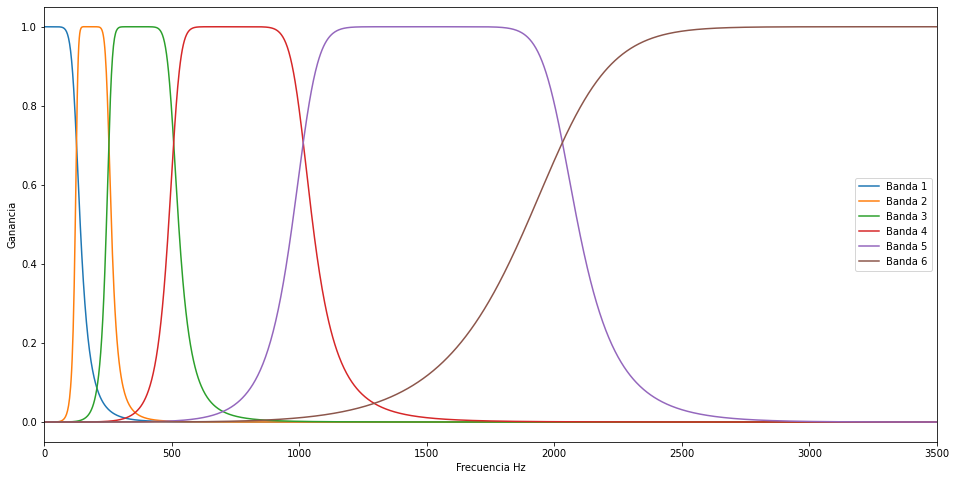
\includegraphics[width=0.9\textwidth]{banco.png}
\caption{Filtros del banco de filtros Butterworth implementado}
\label{bancoresu}
\end{figure}

\newline
En la figura \ref{super} se adjunta la señal a estudiar obtenida del archivo $superstition.wav$, esta señal se filtro con el banco de filtros definido anteriormente y los algunos resultados se presentan en las figuras \ref{low}, \ref{band} y \ref{high} donde se puede ver la selección de la banda de frecuencia correspondiente en el espectrograma y como cambia la forma de la señal temporal. Especialmente en el resultado de la figura \ref{high} se ven los efectos del roll off dado que deja pasar frecuencias desde los $1000Hz$ aproximadamente cuando la frecuencia de corte era $2032Hz$. En el caso de del pasa-bajos se nota claramente la suavización de la señal en el tiempo en contraposición con el resultado de aplicar el pasa-altos. En los casos no incluidos en el informe, los espectrogramas retratan lo mismo que el del pasa-bandas pero en diferentes bandas de frecuencia. En cuanto a la representación temporal, se ve como se va cambiando la apariencia a medida que se va moviendo la banda de observación. 
\begin{figure}[h!]
\centering
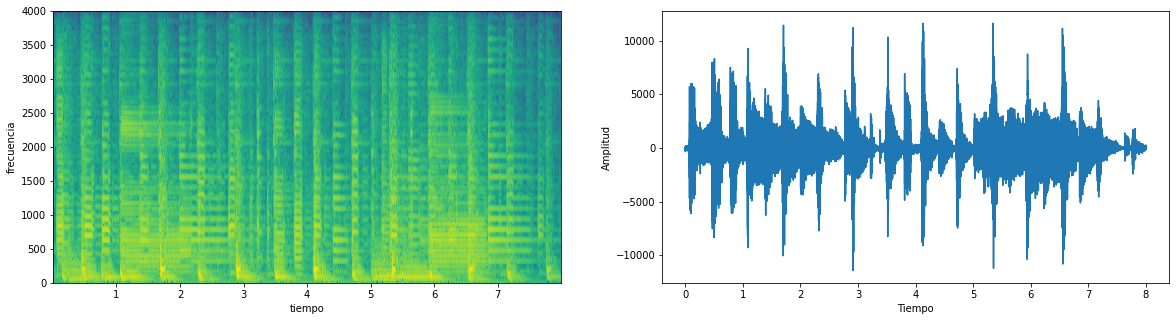
\includegraphics[width=0.9\textwidth]{superstition.png}
\caption{Señal a analizar}
\label{super}
\end{figure}
\begin{figure}[h!]
\centering
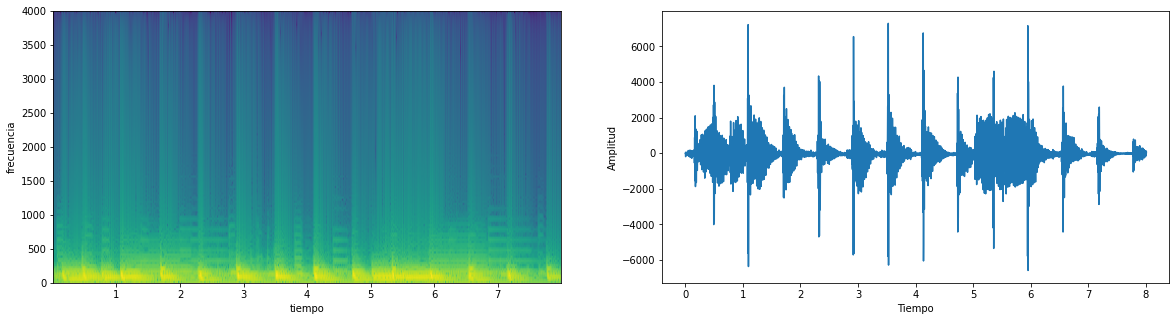
\includegraphics[width=0.9\textwidth]{lowpass.png}
\caption{Señal con el filtro 1 de la tabla \ref{bancoresu}}
\label{low}
\end{figure}
\begin{figure}[h!]
\centering
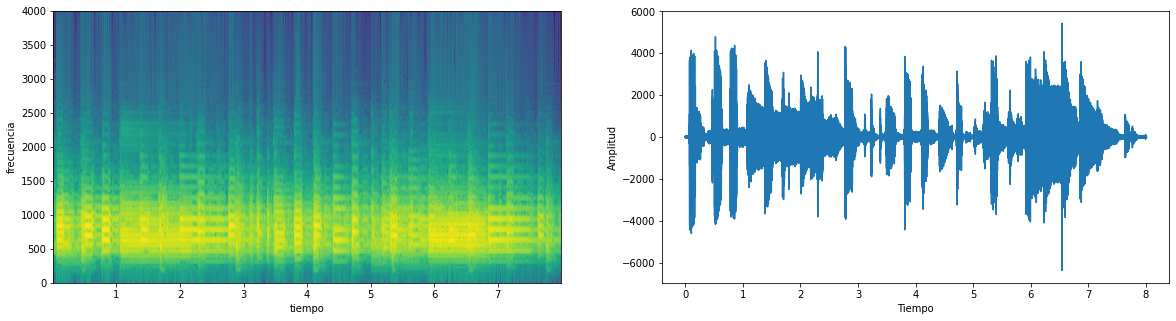
\includegraphics[width=0.9\textwidth]{bandpass4.png}
\caption{Señal con el filtro 4 de la tabla \ref{bancoresu}}
\label{band}
\end{figure}
\begin{figure}[h!]
\centering
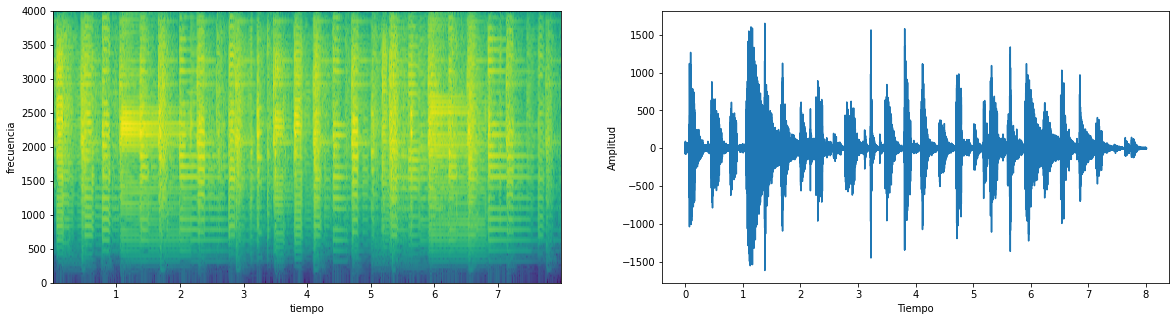
\includegraphics[width=0.9\textwidth]{highpass.png}
\caption{Señal con el filtro 6 de la tabla \ref{bancoresu}}
\label{high}
\end{figure}

\newline
Luego se obtuvo la envolvente de las diferentes señales luego de ser pasadas por cada filtro del banco de filtros. Para obtener la envolvente se rectifico tomando el valor absoluto y luego, siguiendo el procedimiento en \cite{Scheirer} se filtro con un pasa-bajos de frecuencia de corte $10Hz$.
\newline
Luego se creo una señal de ruido blanco de media nula y desviación unitaria para filtrarla con el banco de filtros diseñado anteriormente. Estas bandas de ruido se utilizaron para modular cada banda de la señal original obteniendo así una representación del contenido rítmico en cada banda. Escuchando la modulación de cada banda por separado se percibe que al irse moviendo de banda se escucha mas marcado el ritmo pero al costo de tener mas presencia de ruido. 
\newline
Al sumar todas las señales moduladas se obtiene el resultado final en donde a pesar de la gran presencia de ruido, se puede escuchar el contenido rítmico de la señal original.
\newline
Luego se repitió este procedimiento pero se considero un nuevo banco de filtros presentado en la tabla \ref{papas} para dividir el espectro en un menor numero de bandas.
\begin{table}[h]
\centering
\begin{tabular}{llll}
Banda & f\_low Hz & f\_high Hz & Tipo \\
1 & - & 254 & Lowpass \\
2 & 254 & 1016 & Bandpass \\
3 & 1016 & - & Highpass
\end{tabular}
\caption{Nuevo banco de filtros}
\label{papas}

\end{table}

\subsection{Parte 2}
\newline 
La diferencia con este banco de filtros parece ser que tan ''marcados'' se escuchan los sonidos, con el primer caso se escuchaba mucho mas mientras que en este el contenido rítmico se pierde un poco entre el ruido comparado con el resultado obtenido con el banco de filtros original. Sin embargo esta diferencia es en comparación con el primer banco donde se escucha mejor, pero igual se logra obtener el contenido rítmico de manera relativamente decente. 


\section{Ejercicio 2}
Implementación del algoritmo de Karplus y Strong para síntesis de cuerda pulsada.
\subsection{Parte 1}
El algoritmo se basa en la utilización de filtros peine por lo que en primera instancia se estudiara su respuesta al impulso y sus características.
\newline
El filtro peine tiene el diagrama de bloques de la figura  \ref{peine}, mirando ese diagrama se obtiene que la ecuación en recurrencia es
$$
y[n]=x[n]+R^Ly[n-L]
$$
la frecuencia fundamental de la respuesta al impulso es 
$$
f_0 = \frac{f_S}{L}
$$
con este resultado identificamos un problema, dado que $L\in\mathbb{Z}$ se pueden generar frecuencias fundamentales limitadas, es decir no es posible generar una frecuencia fundamental arbitraria. Esto se puede solucionar agregando un filtro pasa-todos como se vera en la parte 3.
\begin{figure}[h!]
\centering
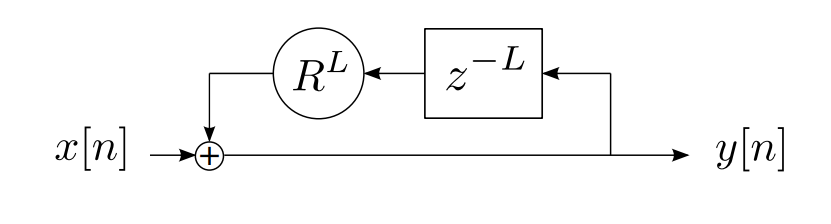
\includegraphics[width=0.9\textwidth]{peine.png}
\caption{Diagrama de bloques del filtro peine \cite{of8}}
\label{peine}
\end{figure}

\newline
El objetivo ahora es sintetizar las 12 notas de una octava en una escala igualmente temperada comenzando en $220Hz$. Para eso en primer lugar se calcularon los valores de L para cada frecuencia utilizando la función round, estos se presentan en la tabla \ref{Ls}.

\begin{table}[!h]
\centering
\resizebox{\textwidth}{!}{%
\begin{tabular}{lllllllllllll}
fobjetivo (Hz) & 220 & 233.08 & 246.94 & 261.63 & 277.18 & 293.66 & 311.13 & 329.63 & 349.23 & 369.99 & 391.99 & 415.30 \\
L      & 100 & 95     & 89     & 84     & 80     & 75     & 71     & 67     & 63     & 60     & 56     & 53    
\end{tabular}%
}
\caption{L para que la frecuencia sea la mas cercana a la deseada}
\label{Ls}
\end{table}

\newline
Luego de encontrar los valores de L se filtra un impulso con cada filtro y se generan señales de 1s correspondientes a cada frecuencia que luego se concatenan en una misma señal de 12s. Las características de la señal resultante van a depender del parámetro R elegido. Para que el filtro sea estable $R^L$ debe ser estrictamente menor a 1 por lo que en definitiva se necesita que $R<1$. La influencia de $R$ se ve directamente escuchando la señal para distintos valores del parámetro, cuando este es menor a aproximadamente $0.9$ no se escucha nada y para valores de $0.9$ y $0.99$ se escuchan ruidos puntuales y aislados. Esto se ve representado en las figuras \ref{09} y \ref{094} donde se ve claramente la ausencia de componentes en las bandas blancas de la figura de la izquierda. Esto es causado por como es la respuesta al impulso de este filtro, 
$$
h[n] = 
\begin{cases}
R^{kL} & \text{si n = kL}\\
0 &\text{en otro caso}
\end{cases}
$$
el $L$ mas chico es 53, se necesita que $R$ sea lo mas grande posible sin salirse de la estabilidad para que se pueda ver/escuchar algo. Esto es porque lo que se esta escuchando es la respuesta al impulso, por lo que se esta escuchando una secuencia de impulsos que decae con el parámetro R, cuanto mas cerca se esta de 1 mas lento decae por lo que el problema es que con R chico decae tan rápido que o no se escucha nada o se escucha una especie de ruido ''puntual''.
\begin{figure}[h]
\begin{minipage}[b]{0.5\linewidth}
\centering
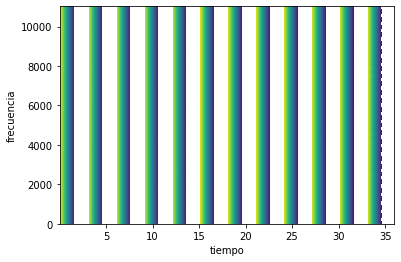
\includegraphics[width=\linewidth]{09.png}
\caption{Espectrograma con $R=0.9$}
\label{09}
\end{minipage}
\hspace{0.5cm}
\begin{minipage}[b]{0.5\linewidth}
\centering
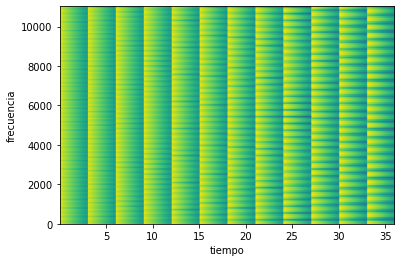
\includegraphics[width=\linewidth]{09999.png}
\caption{Espectrograma con $R=0.9999$}
\label{094}
\end{minipage}
\caption{Comparación de espectrogramas para diferentes Rs}
\label{comparacion1}
\end{figure}

\newline
El resultado obtenido no es bueno, auditivamente no hay parecido con como debería sonar una cuerda pulsada, esto se debe en primer lugar a nuestra falla con los valores de $L$ que podemos tomar, es decir en primer lugar es un problema de resolución que se intentara solucionar en la parte 3, en segundo lugar otro problema es que en una cuerda real los componentes de frecuencia decaen a diferentes velocidades, acá todos los componentes están decayendo con la misma velocidad, $R^L$ en L muestras, pero en una cuerda pulsada las altas frecuencias deberían caer mucho mas rápido que las bajas, esto se intentara arreglar en la parte 2. 

\subsection{Parte 2}
Como primer manera de refinar el modelo se agrega un filtro pasa-bajos en el lazo de realimentación.
Como se venia explicando en la parte anterior, una razón por la cual suena tan mal la primer aproximación realizada es que todos los componentes decaen a la misma velocidad, esto se solucionara agregando un pasa-bajos de acuerdo a \cite{KS} y \cite{Steiglitz}.

\newline
El diagrama de bloques de la figura \ref{bloques2} refleja esta adición. Tomando la señal auxiliar $A[n]$ que seria la entrada al sector punteado de la figura \ref{bloques2}, se tiene que $y[n] = \frac{1}{2}A[n]+\frac{1}{2}A[n-1]$ por lo que la ecuación de recurrencia total es

$$
y[n] = \frac{1}{2} \big[x[n]+R^Ly[n-L]+x[n-1]+R^Ly[n-L-1]\big]
$$

y la frecuencia fundamental de la respuesta al impulso es 
$$
f_0 = \frac{f_S}{L+\frac{1}{2}}
$$
ya que el retardo del bucle no es $L$, es $L+retardo\-pasa\-bajos$ y el retardo que introduce el pasa-bajos es $\frac{1}{2}$.

\begin{figure}[h!]
\centering
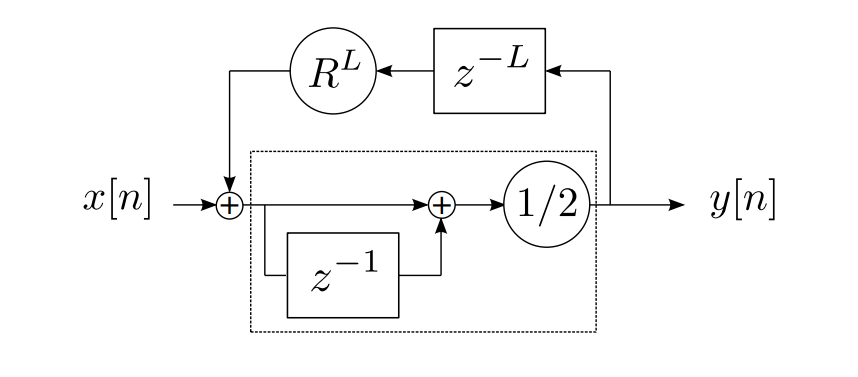
\includegraphics[width=0.9\textwidth]{bloques.png}
\caption{Diagrama de bloques con pasa bajos \cite{of8}}
\label{bloques2}
\end{figure}

\newline
Al igual que en la parte anterior, dada la expresión para la frecuencia fundamental se puede encontrar el valor de $L$ que da la frecuencia mas cercana a la exacta de la escala igualmente temperada utilizando la función round. Los resultados se presentan en la tabla \ref{ls2}.

\begin{table}[!h]
\centering
\resizebox{\textwidth}{!}{%
\begin{tabular}{lllllllllllll}
fobjetivo (Hz) & 220 & 233.08 & 246.94 & 261.63 & 277.18 & 293.66 & 311.13 & 329.63 & 349.23 & 369.99 & 391.99 & 415.30 \\
L      & 100 & 94     & 89     & 84     & 79     & 75     & 70     & 66     & 63     & 59     & 56     & 53    
\end{tabular}%
}
\caption{L para que la frecuencia sea la mas cercana a la deseada con filtro pasa-bajos}
\label{ls2}
\end{table}

\newline
Luego se volvió a repetir el procedimiento de la parte anterior pero con la nueva función que filtra los impulsos con la ecuación en recurrencia que tiene en cuenta el filtro pasa-bajos.
\newline
Luego de concatenar todas las señales obtenidas se obtiene una nueva señal que genera un sonido muy parecido al de una curda pulsada. Lo que resta por hacer es un nuevo refinamiento que genere una mejor afinación en cuanto a las frecuencias fundamentales que se pueden representar. 

\subsection{Parte 3}
Para obtener la escala temperada al valor exacto, es necesario agregar un filtro que no altere la magnitud pero que permita aplicar un retardo fraccionario que se pueda elegir. Para esto se agrega un filtro pasa-todo en serie con el filtro pasa-bajos. El diagrama de bloques para esta implementación se adjunta en la figura \ref{bloquesfinal}.

\begin{figure}[h!]
\centering
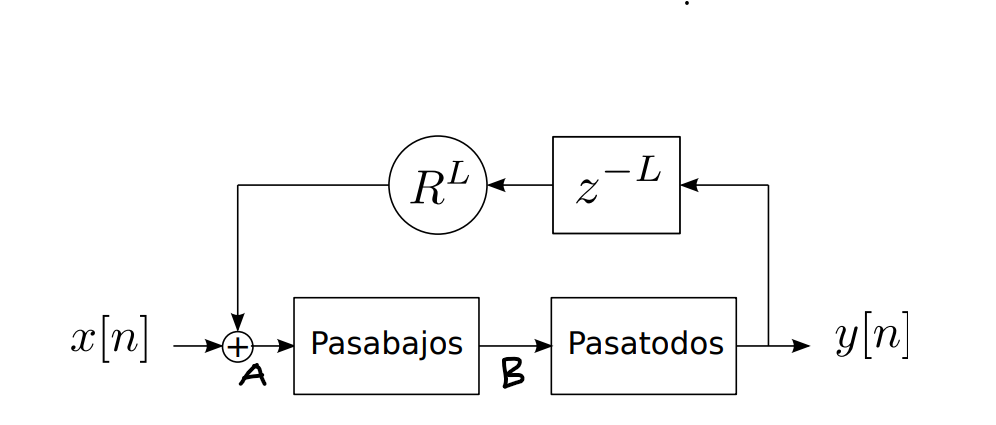
\includegraphics[width=0.9\textwidth]{final.png}
\caption{Diagrama de bloques con pasa bajos y pasa todo \cite{of8}}
\label{bloquesfinal}
\end{figure}

\newline
Tomando los nombres de las señales incluidos en la figura \ref{bloquesfinal} la ecuación de recurrencia del pasa-bajos es
$$
B[n] = \frac{1}{2}A[n]+\frac{1}{2}A[n-1] 
$$
el pasa-todos sigue la implementación de la figura \ref{todos} cuya ecuación de recurrencia siguiendo los mismos nombres de la figura \ref{bloquesfinal} es
$$
y[n] = ay[n-1]-aB[n]+B[n-1]
$$

\begin{figure}[h!]
\centering
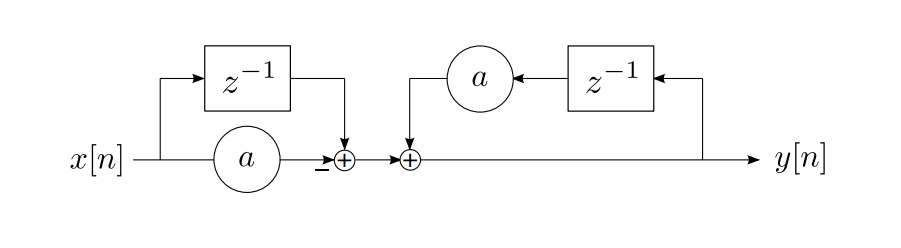
\includegraphics[width=0.9\textwidth]{todos.png}
\caption{Diagrama de bloques de filtro pasa-todo \cite{of8}}
\label{todos}
\end{figure}

\newline
Combinando esas ecuaciones con el lazo del filtro peine se tiene que la ecuación de recurrencia final es
$$
y[n] = ay[n-1] -\frac{a}{2}\big(x[n]+R^ly[n-L]+x[n-1]+R^Ly[n-L-1]\big) + \frac{1}{2}\big(x[n-1]+R^Ly[n-L-1]+x[n-2]+R^Ly[n-L-2]\big)
$$
y tomando el retardo que agrega el pasa todos $\delta = \frac{1+a}{1-a}$ se tiene que la frecuencia fundamental de la respuesta al impulso es
$$
f_0 = \frac{f_S}{L+\frac{1}{2}+\delta}
$$
dado que mientras que $a<1$ se mantiene la estabilidad, el $\delta$ permite obtener la frecuencia fundamental ''exacta''\footnote{Entre comillas porque la realidad es que para llegar a ese retardo se tuvo que realizar una aproximación lineal}. Para implementar esto se eligió un $L$ entero con la función floor del cociente de frecuencias restándose con $\frac{1}{2}$ ya que eso definía un $\delta>0$ que es la diferencia entre el floor y el valor sin truncar. 
\newline
Repitiendo el filtrado pero ahora con esta nueva implementación se obtiene un resultado mas afinado que en la parte anterior.
\newline
Por ultimo se intento estimar el error entre la frecuencia fundamental objetivo y la frecuencia fundamental de la nota para el caso con y sin pasa-bajos. Para realizar este calculo se estimo la frecuencia fundamental de las notas siguiendo la sugerencia de la letra de detectar el primer pico de la DFT dado que la frecuencia fundamental no varia con el tiempo. Los resultados presentan en la tabla \ref{errores}. Los errores están causados por dos razones, la primera es el calculo de la DFT, es decir, hay un error en la estimación de la posición del pico que se puede minimizar aumentando la resolución en el calculo de la DFT. En segundo lugar, para el caso de solo pasa-bajos, se tiene el error directamente de que la frecuencia a la que estamos trabajando no es la buscada exactamente pues el retardo de fase introducido es constante por lo que no nos libera de las consecuencias de que la $L$ que controla la $f_0$ sea un valor entero. Sin embargo, en el caso donde esta el pasa-todos, también hay errores por mas de que se supone que se tenia exactitud, la clave esta en que esa exactitud en realidad viene de una aproximación lineal de la respuesta en fase en bajas frecuencias como se menciona en  \cite{of8}. Por lo que incluso sin errores dados por la estimación de la posición del pico, en ambos casos era esperable que hubiera un error. 

% Please add the following required packages to your document preamble:
% \usepackage{graphicx}
\begin{table}[!h]
\centering
\resizebox{\textwidth}{!}{%
\begin{tabular}{lllllllllllll}
f0objetivo(Hz)        & 220  & 233.08 & 246.94 & 261.63 & 277.18 & 293.66 & 311.13 & 329.63 & 349.23 & 369.99 & 391.99 & 415.30 \\
error sin pasa todos & 0.97 & 0.65   & 0.018  & 0.034  & 0.65   & 1.13   & 1.98   & 2.59   & 2.31   & 0.45   & 2.45   & 3.70   \\
error con pasa todos & 0.5  & 0.64   & 0.018  & 0.034  & 0.64   & 0.33   & 0.51   & 0.34   & 0.63   & 0.44   & 0.49   & 0.70  
\end{tabular}%
}
\caption{Errores de la frecuencia fundamental en cada nota con y sin filtro pasa-todos}
\label{errores}
\end{table}





\newpage
\begin{thebibliography}{100} % 100 is a random guess of the total number of
%references
\addtolength{\leftmargin}{0.2in} % sets up alignment with the following line.
\setlength{\itemindent}{-0.2in}
\bibitem[Scheirer]{Scheirer}Scheirer, E. D. (1998). Tempo and beat analysis of acoustic musical signals. The Journal of the Acoustical Society of America, 103(1).
\bibitem[KarplusStrong]{KS} Karplus, K., & Strong, A. (1983). Digital Synthesis of Plucked String and Drum Timbres. Computer Music Journal, 7(2).
\bibitem[Steiglitz]{Steiglitz} Steiglitz, K. T. (1996). Comb and string filters. In Digital Signal Processing Primer: With Applications to Digital Audio and Computer Music. (1st ed., pp. 101–121). Addison-Wesley.
\bibitem[OF6]{of6} [Introducción a filtros digitales], [Martín Rocamora], Proyecto OpenFING, [https://open.fing.edu.uy/courses/audiodsp/6], publicado bajo una licencia CC By NC ND.
\bibitem[OF7]{of7}[Filtros digitales en audio], [Martín Rocamora], Proyecto OpenFING, [https://open.fing.edu.uy/courses/audiodsp/7], publicado bajo una licencia CC By NC ND.
\bibitem[OF8]{of8}[Aplicaciones en síntesis de sonido y efectos de audio], [Martín Rocamora], Proyecto OpenFING, [https://open.fing.edu.uy/courses/audiodsp/8], publicado bajo una licencia CC By NC ND.
\end{thebibliography}



\end{document}